%Auteurs : Nicolas Englebert
\documentclass[british,french,11pt, a4paper, openany]{book}

% Règles de bonne pratiques :
% https://fr.wikibooks.org/wiki/LaTeX/Gestion_des_gros_documents

\NeedsTeXFormat{LaTeX2e}
\ProvidesPackage{preambule}[5/01/2017 package personnel]

%%%%%%%%%%%%%%%%
%%% Packages %%%
%%%%%%%%%%%%%%%%

%%% Compatibilité %%%
\begingroup\expandafter\expandafter\expandafter\endgroup
\expandafter\ifx\csname IncludeInRelease\endcsname\relax
\RequirePackage{fixltx2e}
\fi 					% Si version LaTeX < 2015, inclut un fix.

%%% Général %%%
\RequirePackage[utf8]{inputenc}
\RequirePackage{babel}
\RequirePackage{lmodern}
\RequirePackage[T1]{fontenc}
\addto\extrasfrench{\sisetup{locale = FR,detect-all}} % Switch siunitx en fonction de la langue babel :)
\addto\extrasbritish{\sisetup{locale = UK,detect-all}}
\addto\captionsfrench{\def\tablename{Tableau}}
\RequirePackage{courier}
\RequirePackage{graphicx}
\RequirePackage[autostyle]{csquotes}

%%% Mise en page %%%
\RequirePackage{mathtools}
\RequirePackage{amssymb}
\RequirePackage{bbm}
\RequirePackage{amsthm}
\RequirePackage{caption}     % Permet d'ajouter des légendes en images sans les mettre en float + dans la marge + ref vers le haut de l'envirronement
\RequirePackage{wrapfig}
\RequirePackage{fullpage}
\RequirePackage{float}      %permet de mettre du texte entre les figures grace a [H]. Génial!
\RequirePackage{eso-pic}    % Fond d'écran page de garde
\RequirePackage{adjustbox}  % Empêche les box de sortir de la page


%%% Math %%%
\RequirePackage{siunitx}

%% Reference
\RequirePackage{hyperref}


%%%%%%%%%%%%%%%%%
%%% Commandes %%%
%%%%%%%%%%%%%%%%%

%%% Physique %%%
\newcommand{\cst}{\text{cst}}
\newcommand{\D}{\partial}
\newcommand{\E}{\vec E}
\newcommand{\B}{\vec B}
\newcommand{\F}{\vec F}
\newcommand{\modu}[1]{|$#1$|}

%%% Math %%%
\newcommand{\oiint}{\int\!\!\!\!\!\!\! \:\!\subset\!\!\supset\!\!\!\!\!\!\!\int}
\newcommand{\rot}{\operatorname{\vec{rot}}}
\newcommand{\divv}{\operatorname{div}}
\newcommand{\phas}[1]{\underline{#1}}
\newcommand{\RE}{\text{Re}}
\newcommand{\ft}{\overset{\mathcal{F}}{\longleftrightarrow}}
\newcommand{\lt}{\overset{\mathcal{L}}{\longleftrightarrow}}
\newcommand{\DS}{\displaystyle}
\newcommand{\Tr}{\operatorname{Tr}}



%% Box
\newcommand{\theor}[1]{\adjustbox{minipage=\linewidth-2\fboxsep-2\fboxrule,fbox}{\textsc{\iflanguage{british}{Theorem}{Théorème}: }#1}}
\newcommand{\defi}[1]{\adjustbox{minipage=\linewidth-2\fboxsep-2\fboxrule,fbox}{\textsc{\iflanguage{british}{Definition}{Définition}: }#1}}
\newcommand{\lemme}[1]{\adjustbox{minipage=\linewidth-2\fboxsep-2\fboxrule,fbox}{\textsc{\iflanguage{british}{Lemma}{Lemme}: }#1}}
\newcommand{\prop}[1]{\adjustbox{minipage=\linewidth-2\fboxsep-2\fboxrule,fbox}{\textsc{\iflanguage{british}{Property}{Propriété}}\\ #1}}
\newcommand{\proposition}[1]{\adjustbox{minipage=\linewidth-2\fboxsep-2\fboxrule,fbox}{\textsc{Proposition}\\#1}}
\newcommand{\cadre}[1]{\adjustbox{minipage=\linewidth-2\fboxsep-2\fboxrule,fbox}{#1}}
\newcommand{\retenir}[1]{\adjustbox{minipage=\linewidth-2\fboxsep-2\fboxrule,fbox}{\textbf{\textit{\textsc{\iflanguage{british}{To remember}{À retenir}}: }}#1}}

\newcommand{\corollaire}[1]{\bigbreak\begin{tabular}{||c}
		\begin{minipage}{\textwidth}
			\textsc{\iflanguage{british}{Corollary}{Corollaire}: } \textit{#1}
		\end{minipage}
\end{tabular}}
\newcommand{\exemple}[1]{\bigbreak\begin{tabular}{|c}
		\begin{minipage}{\textwidth}
			\textsc{\iflanguage{british}{Example}{Exemple}: } #1
		\end{minipage}%
\end{tabular}}%




%%% Background %%%
\newcommand\BackgroundPic{%
	\put(0,0){%
		\parbox[b][\paperheight]{\paperwidth}{%
			\vfill
			\centering
			\includegraphics[width=\paperwidth,height=\paperheight,%
			keepaspectratio]{../../Builder/ulb.jpg}%
			\vfill
}}}

%%% Annexes Cedu %%%
\RequirePackage{fourier-orns}

\setlength{\parindent}{0pt}

%%% Attributs %%%
\newcommand*{\NomduCours}[2]{\def\cours{#1}\def\memo{#2}}
\newcommand*{\annee}[2]{\def\adebut{#1}\def\afin{#2}}

\newcounter{auteurcnt}
\newcommand\addauteur[2]{%
	\stepcounter{auteurcnt}%
	\csdef{auteur\theauteurcnt}{\mbox{#1~\textsc{#2}}}}
\newcommand\getauteur[1]{%
	\csuse{auteur#1}}

\newcounter{illustrateurcnt}
\newcommand\addillustrateur[2]{%
	\stepcounter{illustrateurcnt}%
	\csdef{illustrateur\theillustrateurcnt}{\mbox{#1~\textsc{#2}}}}
\newcommand\getillustrateur[1]{%
	\csuse{illustrateur#1}}

\newcounter{rappeltheocnt}
\newcommand\addrappeltheo[2]{%
	\stepcounter{rappeltheocnt}%
	\csdef{rappeltheo\therappeltheocnt}{\mbox{#1~\textsc{#2}}}}
\newcommand\getrappeltheo[1]{%
	\csuse{rappeltheo#1}}

\newcounter{professeurcnt}
\newcommand\addprofesseur[2]{%
	\stepcounter{professeurcnt}%
	\csdef{professeur\theprofesseurcnt}{\mbox{#1~\textsc{#2}}}}
\newcommand\getprofesseur[1]{%
	\csuse{professeur#1}}

\newcounter{iter}


%Typique Phys
\usepackage{physics}
\usepackage{multicol}

% Attributs
\NomduCours{Physique atomique}{PHYS-H-405}
\addauteur{Nicolas}{Englebert}
\addprofesseur{Michel}{Godefroid}
\annee{2016}{2017}


% Document
\begin{document}
\def\equationautorefname~#1\null{%
	(#1)\null
}
\newcommand{\notes}[1]{\bigbreak\begin{tabular}{|c}
		\begin{minipage}{\textwidth}
			#1
		\end{minipage}%
\end{tabular}}%
%%%%%%%%%%%%%%%%%
% Préliminaires %
%%%%%%%%%%%%%%%%%
\frontmatter
\input{../../Builder/titlepage/titlepage.tex}
\input{../../Builder/APropos.tex}
\tableofcontents
%Si abstract, \input ici

%%%%%%%%%%%%%%%%%%%%%
% Contenu principal %
%%%%%%%%%%%%%%%%%%%%%
\mainmatter

\chapter{Fundamental equations of turbomachinery}

\section{Basics and principles}
\subsection{Introduction}
	About the exam, he likes the drawings and likes to give a sentence and asks if it is the reality or not. The questions are about the \textbf{lectures} and not the notes. This summary is thus mainly based on the lectures. \\

The course is organized as: 

\begin{enumerate}
\item \textbf{Turbopumps} and the system involved: a pump is something  applying pressure to a fluid $\Delta p > 0$, which will first be a liquid $\rho = cst$.

\item \textbf{Turbines:} in this case the fluid involves a pressure loss $\Delta p < 0$, so expansion (a valve, simple releaser). We will see the gas turbines and the hydraulic turbines. Some machines can be used in the two ways, both roles, same mechanical component is acting as a pump and as a turbine in the other direction (reversible). 

\item \textbf{Volumetric compressors:} as in other courses we have polytropic or isentropic efficiency, we can define volumetric compressors. 

\item \textbf{Compressors} $\bm{\rho \neq cst}$: we need to consider the axial and centrifugal systems separately because they are very different and complicated.   
\end{enumerate}


\subsection{Classification of turbomachines}
If the role of the machine is to extract energy from the fluid to the shaft we speak about \textbf{turboproducers} or \textbf{turbomotors} (ex: hydraulic turbines), and in the other case \textbf{turboabsorbers} or \textbf{turbogenerators}. 

\subsection{General organization of turbomachines}
\wrapfig{6}{l}{4}{0.22}{ch1/1} 
We always have a \textbf{shaft}, and on the shaft we have a \textbf{disk} or a \textbf{rotor} where the energy transformation takes place, and on this we put a \textbf{blade} (white rectangle on \autoref{ch1/1}), an element with a given geometry. The blade is situated at a distance $r_H$ from the shaft and implies high tangential velocities. The device is closed by a \textbf{carter} and we have to be careful at the top of the blade since there can be leakage, this is why the clearance is very small ($\mu m$). We can also have active clearance control by blowing fluid on the carter. Remark that there is an \textbf{external carter} (blue 1) and an \textbf{internal carter} (blue 2) that can constitute a convergent distributor and a divergent diffuser. These can contain non rotating parts called \textbf{vane}, we speak of \textbf{vaned convergent}, \textbf{vaned divergent} or \textbf{vaneless} nozzles. The internal carter plays the role of support and is connected to the shaft via \textbf{bearings} and \textbf{seals} (to avoid air preferring this way to reach atmospheric pressure). 

\ \\
\begin{wrapfigure}[7]{l}{4.5cm}
\vspace{-10mm}
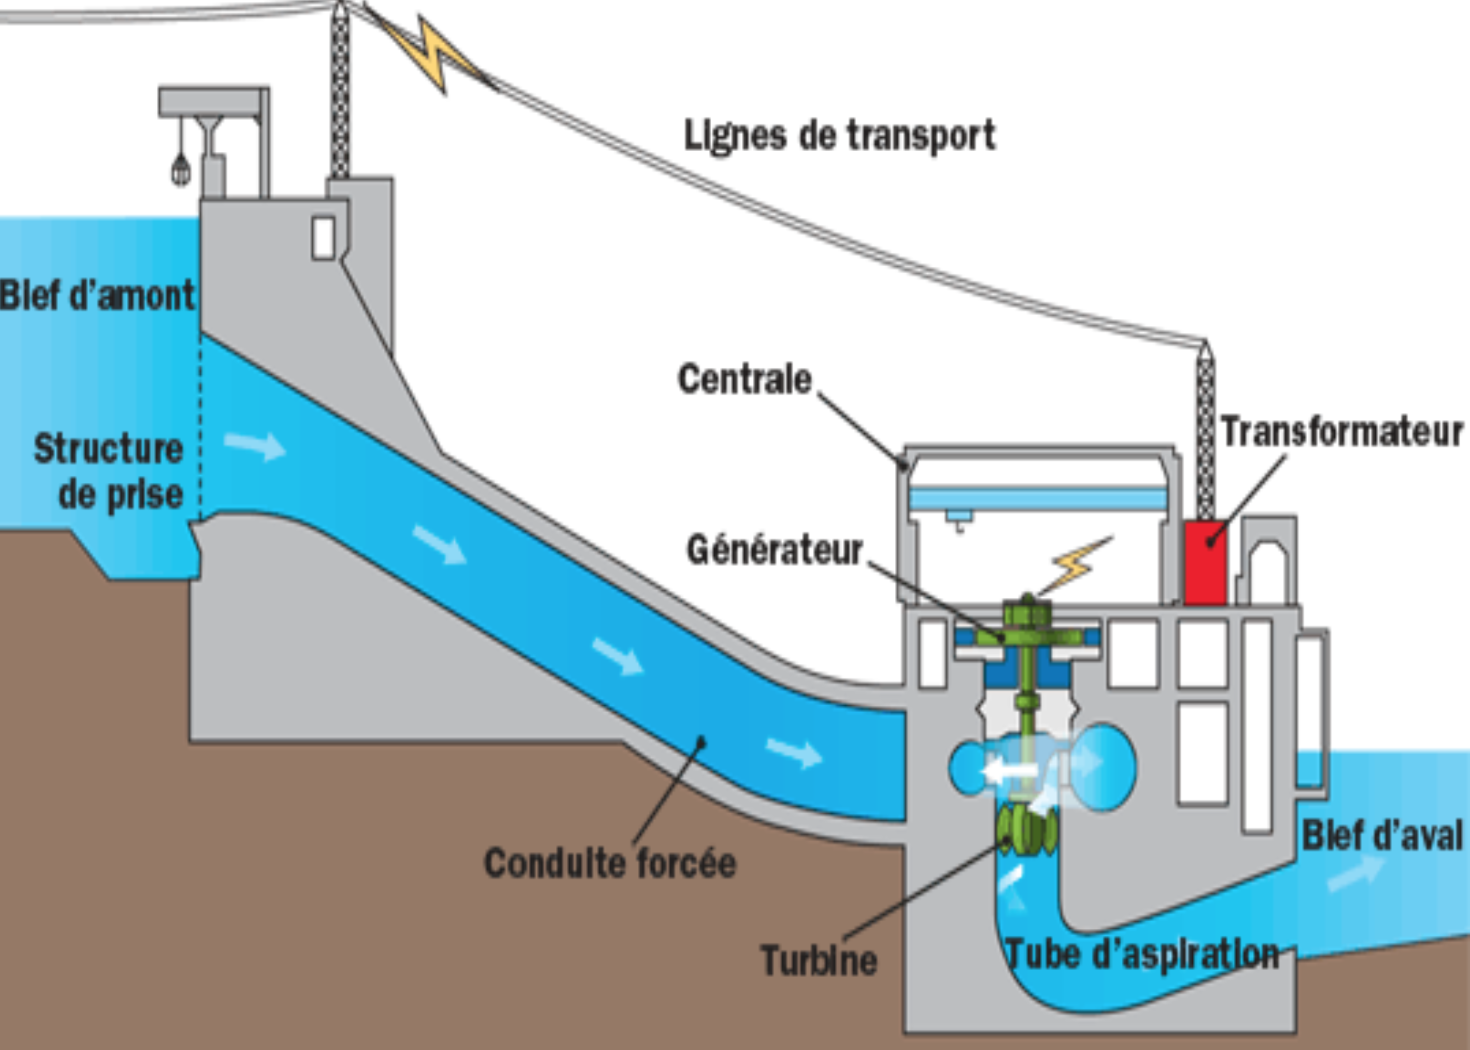
\includegraphics[scale=0.3]{ch1/2}
\captionof{figure}{}
\label{ch1/2}
\end{wrapfigure}
The major types of machine have an axial configuration so that the particles flows parallel to the shaft, radial configuration where flows enters horizontal and leaves vertical also exists. Most turbines or compressors are axial turbines. Turbopumps are most of the time radial, centrifugal. Several disks can be mounted on a same shaft (or several shafts), with fixed components changing the direction of the flow (multistage pump on \autoref{ch1/2}).

\subsection{Notations}
On \autoref{ch1/1}, 0 is the inlet of the distributor, 1 the inlet of the rotor, 2 outlet of the rotor, 3 outlet of the diffuser and i (or e)/o (or s) the upstream/downstream plenum. There are 3 velocity components: the absolute velocity $\bar{v}$, the frame tangential velocity $\bar{u}$ and the relative velocity $\bar{w}$ due to the rotation of fluid particles. 

\subsection{Velocity triangle}
\wrapfig{8}{r}{3.5}{0.3}{ch1/3}
The absolute velocity respects: 

\begin{equation}
\bar{v} = \bar{u} + \bar{w}.
\end{equation}

By defining $\alpha$ and $\beta$ the angle between $\bar{u}$ and respectively $\bar{v}$ and $\bar{w}$, we can write: 

\begin{equation}
v \cos \alpha = u + w\cos \beta \qquad w^2 = u^2 + v^2 - 2uv\cos \alpha
\end{equation}

The velocity triangle is the keypoint of a turbomachine, we have to play with the velocities by means of the mass flow rate $\dot{m}$ and the machine rpm $N$. It is important to see that these parameters are linked to the velocity triangle, for the mass flow for example $\dot{m} = \rho u A$. 


\section{Fundamental equations of the flow}
\subsection{Equations of the flow in a fixed frame}
For all developments, only \textbf{steady state} regime is considered, so that $\omega = cst$ and the flow properties are not time dependent. Moreover, boundary layers are neglected and the flow propagates in parallel slices. 

\subsubsection{Energy equation}
Let's consider sections $A_0$ and $A_1$ denoting the input and output of a non interrupted flow section, for instance 0 to 1 in previous figure. The total energy equation is: 

\begin{equation}
q = h_1 - h_0 + \frac{v_1^2 - v_0^2}{2} + g(z_1-z_0)
\label{2.1}
\end{equation}

where $q$ is the heat exchanged with the outside [J/kg], $v$ is the absolute velocity [m/s] and $h$ is the enthalpy [J/kg]. In adiabatic systems $q=0$. We see that if there is thermal, kinetic or potential energy loss, it will produce heat. Be careful that this equation is not applicable around the blade. 

\subsubsection{Equation of kinetic energy}
We know that kinetic and potential energy can be transformed into work in a machine. We have:

\begin{equation}
 \frac{v_1^2 - v_0^2}{2} + g(z_1-z_0) = - \int _{p_0}^{p_1} \nu dp - w'_f
 \label{2.2}
\end{equation}

where $\nu = 1/\rho$ is the specific volume [$m^3$/kg] and $w'_f$ the work resulting from all friction effects [J/kg]. We see that if velocity increases/decreases, pressure decreases/increases and the friction is a loss, so "-" signs. 

\subsubsection{Global thermodynamic equation}
By considering \eqref{2.2} in \eqref{2.1}: 

\begin{equation}
q + w'_f = h_1 - h_0  - \int _{p_0}^{p_1} \nu dp
\end{equation}

The physical content is different, we see that in fact the losses corresponds to pressure and temperature losses. 

\subsubsection{Mass flow rate equation}
The mass flow is constant over a tube: 

\begin{equation}
\dot{m} = \rho v A = \rho_0 v_0 A_0 = \rho_1 v_1 A_1 = \frac{v_1 A_1}{\nu _1}  
\end{equation}

where $\dot{m}$ [kg/s].

\subsection{Equations of the flow in a moving frame}
Now we can consider the indices 1 and 2 referring to the blade space. 

\subsubsection{Equation of kinetic energy in a relative space}
He skipped the long demo page 8. The equations are the same as before, the only difference is that we replace the absolute velocity by the relative one and an additional kinetic energy term due to the rotation of the frame: 

\begin{equation}
 \frac{w_2^2 - w_1^2}{2} + g(z_2-z_1) = - \int _{p_1}^{p_2} \nu dp - w^"_f + \frac{u_2^2-u_1^2}{2}
 \label{2.5}
\end{equation}

Remark that this term can play a huge role because in a centrifugal system the term is non zero while it is zero in an axial system. 

\subsubsection{Global thermodynamic equation}
The equation is exactly the same as before, except $w'_f$ that becomes $w^"_f$. 
\begin{equation}
q + w^"_f = h_2 - h_1 - \int _{p_1}^{p_2} \nu dp
\end{equation}

\subsubsection{Energy equation}
If we combine the two previous equation we get: 

\begin{equation}
q + \frac{u_2^2-u_1^2}{2} = h_2 - h_1 + \frac{w_2^2 - w_1^2}{2} + g(z_2-z_1)
\end{equation}

\subsubsection{Mass flow equation rate equation}
For a section normal to the relative velocity:

\begin{equation}
\dot{m} = \rho w A = \rho _1 w_1 A_1 = \rho _2 w_2 A_2
\end{equation}


\section{Fundamental equations of turbomachinery}
\subsection{Compressors}
\subsubsection{Internal losses}
\wrapfig{8}{l}{5}{0.3}{ch1/4}
Several kind of losses are present in a compressor. First of all, friction in the distributor gives birth to losses noted $w'_f$. Then, the fluid goes through the interblade channel where its energy increases, but a loss due to friction is present $w^"_f$. In addition, the clearance between the blade tip and the carter is non zero and leads to back-flow leakage $\dot{m}_i$ as the pressure upstream is lower. If we denote the mass flow rate through the blades $\dot{m}_R$, we have: 

\begin{equation}
\dot{m}_R = \dot{m} + \dot{m}_i
\end{equation}

A big part of the flow goes then through the diffuser, but a small part escapes from the seal to the outside $\dot{m}_e$. The small gap between the rotor and the internal carter is filled with part of the fluid. Even if this fluid does not contribute to the energy exchanges (stagnation), part of the power supplied to the shaft will dissipate due to fluid friction $P_{fr}$. 

\subsubsection{External losses}
As discussed, part of the flow escapes through the seals. The upstream one is not a problem since the pressure is close to the atmospheric pressure, but for the downstream seal $\dot{m}_e \neq 0$ since the pressure is higher. This will be neglected in the study. The last losses are due to bearings and other mechanical components such as the fuel pump that we all denote in a single absorbed power $P_{fa}$. 

\subsubsection{Energy equation}
\wrapfig{10}{l}{6.5}{0.3}{ch1/7}
Before going through all the losses appearing in the engine, let's have a global view limiting the study region as on the figure. The total energy equation between input and output is: 

\begin{equation}
q + W_{e\rightarrow s} = u_o - u_i + \frac{v_o ^2 - v_i^2}{2} + g(z_o - z_i)
\end{equation}

where we have the heat exchanged with the outside, the work from external forces to the system due to fluid pressure $p_i \nu _i - p_o\nu_o$ and work applied on the shaft $\frac{P - P_{fa}}{\dot{m}} =  \frac{P_i}{\dot{m}}$ equal to the variation of internal energy, kinetic energy and potential energy. Heat exchanges and the height difference in such engine are negligible, by introducing the enthalpy instead of internal energy and fluid pressure, we have: 

\begin{equation}
P_i = P - P_{fa} = \dot{m}\left( h_o - h_i + \frac{v_o^2 - v_i^2}{2} \right) = \dot{m} (h_{t_o} - h_{t_i}) = \dot{m} c_p (T_{t_o} - T_{t_i})
\end{equation}

where the index $t$ denotes the total or stagnation quantities. We conclude that the work transferred through the shaft increases the total energy of the fluid. 

\subsubsection{Equation of kinetic energy}
This adapted to the work $\frac{P_i}{\dot{m}}$ gives: 

\begin{equation}
P_i = \dot{m} \underbrace{\left( \frac{v_o^2-v_i^2}{2} + \int _{i}^{o} \nu dp + g(z_o - z_i)\right)}_{e} + P_f = \dot{m} e + P_f
\end{equation}

$P_f$ is the internal friction loss with the active as well as the non-active fluid and $e$ is the energy transferred to the fluid. 

\subsubsection{A first distribution of the power - efficiencies}
\wrapfig{7}{r}{3.2}{0.3}{ch1/8}
The figure summarizes all the above equations, for the efficiency we have $\dot{m}e$ at the end and we inject $P$ so: 

\begin{equation}
\eta _{g} = \frac{\dot{m}e}{P} = \frac{\dot{m}e}{P_i} \frac{P_i}{P} = \eta _i \eta _m
\end{equation}

that we rewrite as internal efficiency and external mechanical efficiency. 

\subsubsection{Energy transfer to the rotor}
The only new equation we have is the \textbf{Euler-Rateau equation}. The energy given to the flow in a pump is linked to the energy provided to the shaft. We have to consider the kinetic moment (moment of the quantity of movement) related to the shaft:

\begin{equation}
\frac{d}{dt}\sum M_{axe} (m\bar{v}) = \sum M_{axe}\bar{F}_e
\label{3.2}
\end{equation}

\wrapfig{11}{l}{3}{0.3}{ch1/5}
The variation of the kinetic moment of the rotor is zero since the rotation speed is constant. For a fluid element with mass $m$ and at a distance $r$ of the shaft, the velocity $\bar{v}$ is composed of a component // to the shaft, radial component and tangential component on the rotor. Only the tangential component delivers a moment: 

\begin{equation}
M_{axe}(m\bar{v}) = m r v \cos \alpha 
\end{equation}

and since the flow is permanent, after a time $dt$ very small, if the mass flow is constant: 

\begin{equation}
\sum _{b'b^"} mr v \cos \alpha - \sum _{a'a^"} mr v \cos \alpha = m' (r_2v_2\cos \alpha _2-r_1v_1\cos \alpha _1) = m' (r_2 v_{2u} - r_1 v_{1u})
\end{equation}

Accepting $r_2 v_{2u} - r_1 v_{1u} = cst$ for all channels we get: 

\begin{equation}
\frac{d}{dt}\sum M_{axe}(m\bar{v}) = \frac{d}{dt}\left[(r_2 v_{2u} - r_1 v_{1u}) \sum m'\right] = \dot{m}_R (r_2 v_{2u} - r_1 v_{1u})
\end{equation}

For the right hand side of \eqref{3.2}, the weight of the wheel, the weight of the fluid, the pressures at inlet, at outlet and at side walls are null due to symmetry. Only the \textbf{driving torque} applied on the shaft $\bf{M_i}$ and the \textbf{resistive torque} $-\bf{M_{fr}}$ due to friction between the wheel and the non-active fluid are present, so that we finally get: 

\begin{equation}
\dot{m}_R (r_2 v_{2u} - r_1 v_{1u}) = M_i - M_{fr}
\end{equation}

And if we multiply by $\omega$: 

\begin{center}
\theor{
\textbf{Equation of Euler-Rateau}
\begin{equation}
P_i - P_{fr} = P - P_{fa} - P_{fr} = P_R = \dot{m}_R (u_2 v_{2u} - u_1 v_{1u}) = \dot{m}_R \Delta (uv_u)
\end{equation}
This equation tells that in order to be transferred to the mass flow rate $\dot{m}_R$, the power at the rotor shaft $P_R$ must show an increase of the quantity $uv_u$ which is directly related to the velocity triangle. 
}
\end{center}

As $w^2 = v^2 + u^2 - 2 u v_u$, one can also write: 

\begin{equation}
P_R = \dot{m}_R \left( \frac{v_2 ^2 - v_1^2}{2} + \frac{u_2 ^2 - u_1^2}{2} - \frac{w_2 ^2 - w_1^2}{2} \right)
\label{3.8}
\end{equation}

\subsubsection{Energy generated by the rotor}
Remember \eqref{2.5} and replace this in \eqref{3.8}, we get: 

\begin{equation}
P_R = \dot{m}_R \underbrace{\left( \frac{v_2 ^2 - v_1^2}{2}  + \int _{p_1}^{p_2} \nu dp + g(z_2 - z_1) \right)}_{e_R} + \dot{m} _R w^"_f
\end{equation}

where $e_R$ is the energy transferred to the fluid through the channels on the rotor between section 1 and 2 on the common figure. $\dot{m}_R w^"_f = P^"_f$ being the power absorbed by friction effects, we get: 

\begin{center}
\theor{
\begin{equation}
P_R = \dot{m}_Re_R + P^"_f \qquad \left(\mbox{and } P_R = \dot{m} (h_{t_2} - h_{t_1}) \right)
\end{equation}
}
\end{center}

And we get thus 4 different expression for $P_R$, where the last expression was given in lecture. 

\subsection{Detailed power distribution}
The different losses can be depicted thanks to the previous equation:

\begin{equation}
P_i = P-P_{fa} \qquad P_R = P_i - P_{fr} \qquad \dot{m}_Re_R = P_R - P^"_{f} \qquad \dot{m}_R = \dot{m} + \dot{m}_i
\end{equation}

\wrapfig{12}{l}{5}{0.3}{ch1/6}
where we clearly see the mechanical losses, the loss due to stationary fluid, the loss at the rotor and the back flow. To this we have to add the loss at the diffuser and distributor which we wrote as:

\begin{equation}
P'_f = \dot{m}w'_f
\end{equation}

On the figure, we first see the loss due to mechanical components giving $P_i$, then the fluid losses composed of stationary fluid losses giving $P_R$, then rotor channels loss giving $\dot{m}_Re_R$, but we have the back flow loss $\dot{m}_i e_R$ giving $\dot{m}e_R$ and the last venturi losses that gives the output power $\dot{m}e$ plus all the losses. 

\section{Turbines}
\subsubsection{Description}
\wrapfig{11}{r}{4.5}{0.3}{ch1/9}
The equations are in fact the same except that we have to adapt the signs and indexes to the working principle since the energy is flowing from the fluid to the shaft. As before, there is a clearance flow $\dot{m}_i$ such that: 

\begin{equation}
\dot{m} = \dot{m}_R + \dot{m}_i
\end{equation}

The losses due to mechanical components $P_{fa}$ and the leakage flows $\dot{m}_e$ (negligible), the energy losses in non rotating ($w'_f$) and rotating ($w^"_f$) frame and the loss due to non-active fluid $P_{fr}$ are present. The useful power $P_u$ replaces the $P$ we had before. 

\subsubsection{Energy equation}
It is the same as before except that the indexes are inverted and the useful power is $P_u = P_i - P_{fa}$:

\begin{equation}
P_i = P_u + P_{fa} = \dot{m} (h_{t_i} - h_{t_o})
\end{equation} 

\subsubsection{Equation of kinetic energy}
\begin{equation}
P_i = \dot{m} \underbrace{\left( \frac{v_i^2-v_o^2}{2} + \int _{p_o}^{p_i} \nu dp + g(z_i - z_o)\right)}_{e} - P_f = \dot{m} e - P_f
\end{equation}

\subsubsection{First distribution of the power}
The efficiencies are inverted: 

\begin{equation}
\eta _g = \frac{P_u}{\dot{m}e} = \frac{P_u}{P_i}\frac{P_i}{\dot{m}e} = \eta _m \eta _i
\end{equation}

On \autoref{ch1/10} is represented a first plot of the different powers, remark that it is similar to what we had, only the fluid losses comes before the mechanical losses. The fluid losses are the same as before. 

\minifig{ch1/10}{ch1/11}{0.4}{0.27}{0.35}{0.35}

\subsubsection{Equation of Euler-Rateau}
We can rewrite $P_R$ as the power transfered to the rotor from the fluid $\dot{m}_R$: 

\begin{equation}
P_R = P_i + P_{fr} = \dot{m} _R (u_1v_1\cos \alpha _1 - u_2v_2\cos \alpha _2) 
\end{equation}

\subsubsection{Energy absorbed by the rotor}
As before, combing the above equation and the equation for rotating frame we get: 

\begin{equation}
P_R = \dot{m}_R e_R - P^"_f
\end{equation}


\section{Axial thrust and disc friction}
\subsection{Definition}
Since turbomachines are used to increase the energy of the fluid or extract energy from it, the pressure at the two sides of the rotor is different. This leads to an axial force and we need \textbf{thrust bearings} to avoid the shaft to slip. 

\subsection{Equation of the axial thrust}
\wrapfig{9}{l}{3.5}{0.3}{ch1/12}
We apply the equation of quantity of movements to the wheel and fluid without the shaft between section 1 and 2: 

\begin{equation}
\sum \frac{d}{dt}(m\bar{v}) = \sum \bar{F}_e
\end{equation}

We will make a projection along x-axis. The present external forces are: pressure forces $p_1A_{R1}$ and $p_2A_{R2}$, weight of the rotor and the fluid projected is $G\cos \delta$ and reaction force of the shaft on the rotor with projection $F_{ax}$ so $-F_{ax}$ as seen by the rotor (projection of moments is null). The equation of quantity of movement becomes: 

\begin{equation}
\begin{aligned}
&\dot{m}_R\, (v_{2ax} - v_{1ax}) = p_1 A_{R1} - p_2 A_{R2} + F_{ax} + G\cos \delta \\
\Leftrightarrow\qquad &F_{ax} = \dot{m}_R\, dt (v_{2ax} - v_{1ax}) + P_2 A_{R2} - P_1 A_{R1} -  G\cos \delta
\end{aligned}
\end{equation}

\subsection{Friction of the disc}
\wrapfig{9}{l}{5.5}{0.3}{ch1/13}
As mentioned before, there is friction between the disc and the non-active fluid. It is obvious that the friction torque will increase with the radius (more surface), the rpm ($u$) and the volumetric mass of the fluid. Considering an elementary surface $2\pi r\, dr$, we find experimentally for the elementary friction force and torque: 

\begin{equation}
dF_{fr} = K\rho u^2 2\pi r \,dr \qquad dC_{fr} = 2K\rho 2\pi r^2\, dr\, u^2 
\end{equation}

the 2 appears by considering the 2 sides of the disc. We integrate from internal radius $r$ to the external one $r_1$ and multiply by $\omega$ to have powers (neglect $r^5$ compared to $r_1^5$): 

\begin{equation}
C_{fr} = K\rho \omega ^2 r_1^5 \qquad \Rightarrow P_{fr}= K\rho \omega ^3 r_1^5
\end{equation}

Remark that one could think that we will have enormous values for $\omega ^3$, but be aware that if $\omega$ increases, the mechanical stresses on the device increases and force to reduce the $r_1$. This is why the friction is finite. If the side walls are very smooth, the coefficient K is related to the Reynolds number: 

\begin{equation}
Re = \frac{\rho \omega r_1^2}{\mu}
\end{equation}


\chapter{Interaction matière-lumière}
\section{Équations de Maxwell}
Les équations de \textsc{Maxwell} du champ électrique et du champ d'induction magnétique sont 
désormais bien connue
\begin{equation}
{\bf E} ({\bf r},t) = - \mbox{\boldmath $ \nabla $} \Phi({\bf r},t) - 
  \frac{\partial }{\partial t} {\bf A} ({\bf r},t),\qquad\qquad
  {\bf B} ({\bf r},t) = \mbox{\boldmath $ \nabla $} \times {\bf A} ({\bf r},t)
\end{equation}
La jauge de \textsc{Coulomb} $\vec\nabla.\vec{A}=0$ permet d'imposer des ondes transverses. On obtient
alors l'équation d'onde
\begin{equation}
\nabla ^2 {\bf A} - \frac{1}{c^2} \frac{\partial ^2 {\bf A}}{\partial t ^2} = 0 
\end{equation}
Nous avons en effet $\phi=0$ dans le vide. La solution de cette équation est une onde plane
monochromatique
\begin{equation}
{\bf A}(\omega; {\bf r},t) = {\bf A}_0(\omega) 
   \cos ( {\bf k} \cdot {\bf r} - \omega t  
 + \delta_{\omega} ) 
\end{equation}
où $\vec A_0$ est le vecteur d'amplitude, qui décrit l'intensité et la polarisation de la radiation, $\vec{k}$ est le vecteur de 
propagation ($\omega=kc$) et où $\delta_\omega$ est une phase réelle. Comme annoncé, la jauge de
\textsc{Coulomb} impose
\begin{equation}
\mbox{\boldmath $ \nabla $} \cdot {\bf A} = 0  \; \; \mbox{si} \; \; 
   {\bf k} \cdot {\bf A}_0(\omega) = 0 
\end{equation}
Les ondes sont donc transverses : $\vec{k}\perp\vec{A_0}(\omega)$. Avec ce choix de potentiel vecteur,
nous pouvons ré-écrire le champ électrique, l'induction magnétique 
\begin{equation}
{\bf E} ({\bf r},t)  = E_0(\omega)
\hat{ \mbox{\boldmath $ \epsilon $} } 
  \; \sin ( {\bf k} \cdot {\bf r} - \omega t + \delta_{\omega}),\qquad\qquad
  {\bf B} ({\bf r},t) = E_0(\omega)
\omega^{-1}
 ({\bf k} \times \hat{ \mbox{\boldmath $ \epsilon $}} )
\; \sin ( {\bf k} \cdot {\bf r} - \omega t + \delta_{\omega})
\end{equation}
et le potentiel vecteur
\begin{equation}
 {\bf A}_0(\omega) = A_0(\omega) 
\hat{  \mbox{\boldmath $ \epsilon $}}
\Rightarrow   {\bf k} \cdot 
\hat{  \mbox{\boldmath $ \epsilon $}} = 0
\end{equation}
où $\vec{\hat{\epsilon}}$ est le vecteur de polarisation. Il nous informe la direction dans laquelle
$\vec{A_0}$ pointe. Comme $\vec{E}$ contient également ce vecteur, il est forcément colinéaire à 
$\vec{A_0}$. L'onde est forcément transverse ($\vec{k}\perp\vec{A}$) et la direction de polarisation
de $\vec{E}$ est imposée par $\vec{A}$. Notons qu'il est possible de déterminer un état arbitraire
de polarisation en effectuant la combinaison de deux ondes planes indépendantes. Notons également
que $E_0(\omega) = - \omega A_0(\omega)$.\\

A l'aide du vecteur de \textsc{Poynting} ($\propto |E|^2$), il est possible de déterminer l'intensité
du champ électrique (ou du potentiel vecteur)
\begin{equation}
  I(\omega) 
= \frac{1}{2} \epsilon_0 c E_0^2 (\omega) 
=  \frac{1}{2} \epsilon_0 c \omega^2  A_0^2 (\omega) 
= \frac{\hbar \omega N(\omega) c}{V}
= \rho (\omega) c
\end{equation}
La dernière égalité est le produit de la densité photonique par la vitesse de la lumière. La densité
photonique (ou densité de radiation) s'exprime
\begin{equation}
\rho(\omega) 
= \frac{1}{2} \epsilon_0 E_0^2 (\omega)
= \frac{1}{2} \epsilon_0 \omega^2
A_0^2 (\omega) = \frac{N (\omega) \hbar \omega}{V}
\end{equation}
Cette densité est l'énergie $\hbar\omega$ que porte chaque photon, multiplié par $N(\omega)$ le nombre
de photon, par la vitesse de la lumière $c$ et divisé par le volume. Il s'agit bien d'une énergie par
unité de surface et de temps.\\

Notons les deux relations intégrales suivantes
\begin{equation}
I = \int_0^\infty I (\omega) d\omega \hspace*{1cm};
\hspace*{1cm}
\rho = \int_0^\infty \rho (\omega) d\omega 
\end{equation}
Ces relations sont rencontrée lorsque l'on ne se situe pas dans un cas monochromatique : par exemple,
un \textit{pulse} a une forme dans l'espace et le temps.

\section{Équation de Schrödinger dépendante du temps}
Les solutions des équations de \textsc{Maxwell} pouvant bien évidemment dépendre du temps, il faut se
soucier de l'évolution dans le temps (mais aussi toujours de l'espace) du potentiel vecteur en tenant
compte du fait que ce n'est pas intégralement monochromatique. On défini alors la forme générale d'un
pulse de radiation
\begin{equation}
  {\bf A} ({\bf r}, t) 
= \hat{  \mbox{\boldmath $ \epsilon $}}
\int_{\Delta \omega} A_0 (\omega) 
   \cos ( {\bf k} \cdot {\bf r} - \omega t + 
\delta_{\omega} )  \; d \omega
\end{equation}
L'hamiltonien d'une particule chargée (sans spin) dans un champ électromagnétique s'écrit
\begin{equation}
H = \frac{1}{2m} ({\bf p} - q {\bf A} ) ^2 + q \Phi
\end{equation}
Utilisons celui-ci pour écrire l'équation de Schrödinger dépendante du temps
\begin{equation}
i \hbar \frac{\partial}{\partial t} \Psi ({\bf r}, t)
= \left[ \frac{1}{2m} (-i \hbar  \mbox{\boldmath $ \nabla $} + e {\bf A}) ^2
  - \frac{Ze^2}{(4 \pi \epsilon_0) r } \right] \Psi ({\bf r}, t)
\end{equation}
Comme $\vec\grad A=0$ (jauge de \textsc{Coulomb}), nous avons que
\begin{equation}
 \mbox{\boldmath $ \nabla $} \cdot ({\bf A} \Psi )
= {\bf A} \cdot (  \mbox{\boldmath $ \nabla $} \Psi)
\end{equation}
Il est donc possible de remplacer le double produit par l'un de ces deux termes. A un facteur 2 près,
ça n'a pas d'importance. Ce facteur disparait d'ailleurs dans la forme réécrite ci-dessous
\begin{equation}
i \hbar \frac{\partial}{\partial t} \Psi ({\bf r}, t) =\left[ -\frac{\hbar ^2}{2m} \nabla ^2 - \frac{Ze^2}{(4 \pi \epsilon_0) r } 
  - \underbrace{\frac{i \hbar e}{m} {\bf A} \cdot \mbox{\boldmath $ \nabla $} 
  + \frac{e^2}{2m} {\bf A} ^2}_{(*)} \right] \Psi ({\bf r}, t)
\end{equation}
La ré-écriture fait apparaitre deux termes (marqués par $(*)$) dans l'Hamiltonien. Ceux-ci sont 
négligeable, il est nécessaire que l'intensité soit faible (car $I = f(\vec{A})$).\\

On peut considérer que l'on se trouve dans un cas de champs faibles si
\begin{equation}
  {\bf A}^2 \ll {\bf A}
\end{equation}
L'exclusion des termes en $A^2$ signifie que l'on est contraint de considérer le cas ou nous avons
l'émission ou l'absorption d'un seul photon à la fois (le bas bi-photonique ne peut pas être traité
sous cette hypothèse). Sous celle-ci, l'équation de Schrödinger dépendante du temps s'écrit plus
simplement
\begin{equation}
i \hbar \frac{\partial}{\partial t} \Psi  = [ H_0 + H'(t)] \Psi
\end{equation}
où $\DS H_0 = -\frac{\hbar ^2}{2m} \nabla ^2 - \frac{Ze^2}{(4 \pi \epsilon_0) r }$ et 
$\DS H'(t) = - \frac{i \hbar e}{m} {\bf A} \cdot \mbox{\boldmath $ \nabla $}$.\\

Pour résoudre cette équation, nous allons introduire la \textit{théorie des perturbations dépendantes
du temps}. Supposons que l'on ai résolu le problème aux valeurs propres $H_0 \psi_k = E_k \psi_k$. 
Nous pouvons alors écrire 
\begin{equation}
\Psi = \sum_k c_k(t) \psi_k ({\bf r}) e^{-iE_kt/\hbar}
\end{equation}
En insérant cette équation dans celle de Schrödinger écrite ci-dessus, on trouve l'expression 
analytique exacte suivante
\begin{equation}
 \dot{c}_b(t) = \frac{1}{i \hbar} \sum_k H'_{bk} (t) c_k (t) e^{i \omega_{bk} t }
\end{equation}
Pour que cette expression ai un sens, il faut que $H'$ puisse couplet l'état $n$ et l'état $k$ sur
lequel porte la somme afin d'avoir un transfert de population d'n état non-perturbé vers une somme
d'états perturbés
\begin{equation}
 H'_{bk} (t) = \langle \psi_b \vert H'(t) \vert \psi_k \rangle,\qquad\qquad
 \omega_{bk} = (E_b - E_k) / \hbar
\end{equation}
La perturbation va donc peupler d'autres état par implication même de cette perturbation.\\

Hélas, cette équation \textit{exacte} n'est pas ré-solvable. Il est nécessaire d'introduire une 
condition initiale stipulant qu'initialement, le seul état peuplé est $a$
\begin{equation}
\Psi (t=0) = \psi_a  \Rightarrow  c_k (t \leq 0) = \delta_{ka} 
\end{equation}
La théorie des perturbations à l'ordre un nous donne
\begin{equation}
c_b^{(1)} (t) = \frac{1}{i \hbar} \int_0^t H'_{ba}(t') e^{i \omega_{ba} t' } dt'
= -\frac{e}{m} \int_0^t 
   \langle \psi_b \vert {\bf A} \cdot \mbox{\boldmath $ \nabla $}  \vert \psi_a \rangle
   e^{i \omega_{ba} t' } dt'
\end{equation}
Le potentiel vecteur est lui donné par
\begin{equation}
  {\bf A} ({\bf r}, t) 
= \hat{  \mbox{\boldmath $ \epsilon $}}
\int_0^\infty A_0 (\omega) 
   \cos ( {\bf k} \cdot {\bf r} - \omega t + 
\delta_{\omega} )  \; d \omega
\end{equation}
où $\omega$ est la fréquence atomique. En substituant cette expression
\begin{equation}
\begin{array}{ll}
 c_b^{(1)} (t) = \DS&\DS-\frac{e}{2m} 
\int_0^\infty d\omega A_0(\omega)\times \left[ e^{i \delta_{\omega}} 
  \langle \psi_b \vert e^{i {\bf k} \cdot {\bf r} }
  \hat{  \mbox{\boldmath $ \epsilon $}} \cdot \mbox{\boldmath $ \nabla $}
  \vert \psi_a \rangle \int_0^t dt' e^{i(\omega_{ba} - \omega) t' } \right.\vspace{2mm}\\
\DS    &\DS+\left. e^{-i \delta_{\omega}} 
  \langle \psi_b \vert e^{-i {\bf k} \cdot {\bf r} }
  \hat{  \mbox{\boldmath $ \epsilon $}} \cdot \mbox{\boldmath $ \nabla $}
  \vert \psi_a \rangle \int_0^t dt' e^{i(\omega_{ba} + \omega) t'} \right]
\end{array}
\end{equation}
où $|c_b^{(1)}|^2$ est la probabilité de trouver $\omega=\omega_{ba}$, $\omega=-\omega_{ba}$ ou
les deux. Nous voyons apparaître un terme de phase où l'on retrouve dans les termes de phase la
fréquence de l'opérateur $\omega$ (fréquence atomique) mais aussi $\omega_{ba} = \omega_b-\omega_a$
(soit une "différence d'énergie") qui peut être négative.\\

Globalement, il existe deux possibilités : $\omega=\omega_{ba}$ ou $\omega=-\omega_{ba}$. En fonction
de la possibilité, un des deux termes "entre crochet" va s'annuler\footnote{En réalité, en prenant 
le module carré, il y aura un terme d'interférences. On peut montrer que celui-ci est  négligeable, 
nous ne le prendrons pas en compte}.\\

\cadre{\begin{description}
\item[Absorption] La première intégrale sur $t'$ est négligeable, sauf si
\begin{equation}
 \omega_{ba} \approx \omega \rightarrow E_b \approx E_a + \hbar \omega
\end{equation} 
\item[Émission] La seconde intégrale sur $t'$ est négligeable, sauf si
\begin{equation}
\omega_{ba} \approx - \omega \rightarrow E_b \approx E_a - \hbar \omega
\end{equation}
\end{description}}\ \\

Il s'agit de deux phénomènes stimulés, nous aurons l'occasion d'en reparler. La première 
condition $\omega = \omega_{ba}$ est la \textit{condition de résonance de Bohr} : il faut que
le photon ai juste l'énergie entre les deux états pour que ça puisse se produire. Savoir quel terme
"survit" c'est bien, mais il reste à calculer l'intégrale.\\

Afin de ne pas faire de recopiage inutile, renommons l'élément de matrice
\begin{equation}
M_{ba} \equiv  \langle \psi_b \vert e^{i {\bf k} \cdot {\bf r} }
  \hat{  \mbox{\boldmath $ \epsilon $}} \cdot \mbox{\boldmath $ \nabla $} \vert \psi_a \rangle
\end{equation}
Il s'agit en réalité de l'\textit{élément de couplage}. Sous cette notation, le module carre discuté
ci-dessus s'écrit
\begin{equation}
  \vert c_b^{(1)} (t) \vert ^2 = \frac{1}{2}
\left( \frac{e}{m} \right) ^2
 \int_0^\infty d \omega
  A_0 (\omega) ^2
    \vert M_{ba} (\omega) \vert ^2 \; F(t,\omega - \omega_{ba} )
\end{equation}
où $A_0$ est une amplitude proportionnelle à l'intensité du champ et $F$ est une fonction dépendante
du temps $t$
\begin{equation}
F(t,\tilde{\omega}) \equiv F(t,\omega - \omega_{ba}) 
= \frac{1 - \cos \tilde{\omega} t }{\tilde{\omega}^2}
\end{equation}
Le résultat de l'intégrale de $F$ est bien connu
\begin{equation}
\int_{-\infty}^{+\infty}
F(t, \tilde{\omega}) d\tilde{\omega} = t 
\int_{-\infty}^{+\infty} \frac{\sin^2 x }{x^2} dx = \pi t
\end{equation}

	\begin{wrapfigure}[10]{r}{5cm}
	\vspace{-5mm}
	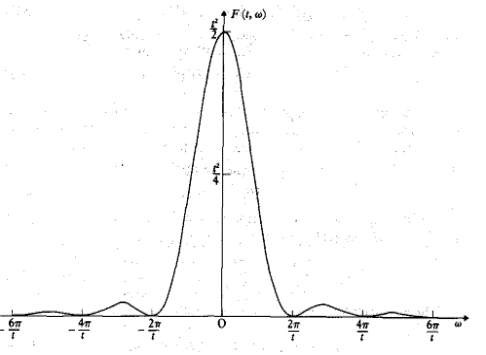
\includegraphics[scale=0.4]{ch2/image1}
	\captionof{figure}{ }
	\end{wrapfigure}
Ci-contre, une représentation de $F(t,\tilde{\omega})$. Il ne s'agit pas d'un delta de \textsc{Dirac}.
Par contre, sous l'approximation du temps long, la largeur du pulse devient suffisamment mince que
pour considérer que c'est le cas
\begin{equation}
F(t \rightarrow \infty, \tilde{\omega}) \sim \pi t \; \delta(\tilde{\omega})
\end{equation}
Revenons au calcul précédent en utilisant ce résultat pour l'intégration sur tous les
$\tilde{\omega}$
\begin{equation}
  \vert c_b^{(1)} (t) \vert ^2 = 
\frac{1}{2} \left( \frac{e}{m} \right) ^2
A_0^2 (\omega_{ba}) 
     \vert M_{ba} (\omega_{ba}) \vert ^2 \; 
\underbrace{\int_{-\infty}^{+\infty}
F(t, \tilde{\omega}) d \tilde{\omega}}_{\pi t}
\end{equation}
On trouve alors que la probabilité augmente \textbf{linéairement} avec $t$ \\

\cadre{\begin{equation}
\vert c_b^{(1)} (t) \vert ^2 = \frac{\pi}{2}
 \left[ \frac{e A_0 (\omega_{ba})}{m} \right] ^2
    \vert M_{ba} (\omega_{ba}) \vert ^2 \; t
\end{equation}}\ \\

Il s'agit d'une nouvelle condition de résonance nous informant sur le fait que $\omega$ doit
être proche de $\omega_{ba}$.\footnote{A vérifier.}

\section{Absorption et émission stimulées}
La probabilité d'\textbf{absorption} s'obtient en dérivant temporellement le module carré calculé 
ci-dessus
\begin{equation}
W_{b \leftarrow a} =
\frac{d}{dt} \vert c_b^{(1)} (t) \vert ^2 =
\frac{\pi}{2} \left[ \frac{e A_0 (\omega_{ba}) }{m} \right] ^2 
\vert M_{ba} (\omega_{ba}) \vert ^2
\end{equation}
En reprenant le lien entre $A_0$ est $I$ (en début de chapitre, avec le vecteur de \textsc{Poynting})
\begin{equation}
W_{b \leftarrow a} =\frac{4 \pi ^2}{m^2 c} \left( \frac{e^2}{4 \pi \epsilon_0 } \right)
\frac{I( \omega_{ba}) }{\omega_{ba}^2 } \vert M_{ba} (\omega_{ba}) \vert ^2
\end{equation}
Cette probabilité sera  non nulle lorsque l'élément matriciel $M_{ba}$ est nul nul. Ceci met en 
évidence la quantification de la matière par l'atome d'hydrogène. L'interaction lumière-matière sera
traitée de façon semi-classique. \\

Il existe un effet symétrique inverse à celui-ci : $\tilde W_{b\leftarrow a}=W_{b\leftarrow a}$. Ce
phénomène est l'\textbf{émission stimulée} dont la probabilité est donné par
\begin{equation}
\tilde{W}_{a \leftarrow b} = \frac{4 \pi ^2}{m^2 c} \left( \frac{e^2}{4 \pi \epsilon_0 } \right)
\frac{I( \omega_{ba}) }{\omega_{ba}^2 } \vert \tilde{M}_{ab} (\omega_{ba}) \vert ^2
\end{equation}
En définissant l'élément de matrice
\begin{equation}
\tilde{M}_{ab} = \langle \psi_a \vert e^{-i {\bf k} \cdot {\bf r} }
  \hat{  \mbox{\boldmath $ \epsilon $}} \cdot \mbox{\boldmath $ \nabla $} \vert \psi_b \rangle
\end{equation}
En comparant cet élément matriciel au précédent, c'est sans surprise que l'on retrouve
\begin{equation}
\tilde{M}_{ab} = - M_{ba}^{\ast} \Rightarrow \tilde{W}_{a \leftarrow b} = W_{b \leftarrow a}
\end{equation}
La seule différence par rapport au cas précédent se situe donc dans l'élément de matrice. Les 
populations $a$ et $b$ ne seront pas peuplées de la même façon. Selon \textsc{Boltzmann}, la 
population dépend de l'énergie ($N\propto g_ie^{-E/kT}$). Si l'on tient compte de ce facteur 
de proportionnalité, il y a plus de change d'observer une absorption qu'une émission stimulé. Ceci
n'est évidemment pas le cas dans des dispositifs comme les \textit{laser} où il y a eu inversion 
de la population, mais rappelons que cette situation ne décrit pas un équilibre thermodynamique.



\section{Le photon QED et l'émission spontanée}
Nous avons jusqu'ici suivi une approche semi-classique. En passant par le théorie quantique des 
champs, nous allons essayer d'estimer l'erreur faite (section informative si j'ai bien compris). 

\subsection{Absorption d'un photon à partir d'un état à $N$ photons}
En quantifiant le champ électrique, on retrouve un potentiel vecteur ayant exactement la même forme
que précédemment
\begin{equation}
  {\bf A}_1 = 
  \hat{  \mbox{\boldmath $ \epsilon $}}
\left[  \frac{2 N(\omega) \hbar}{ V \epsilon_0 \omega}
  \right] ^{1/2} \frac{1}{2}
  \exp [ i ( {\bf k} \cdot {\bf r} - \omega t 
+ \delta_{\omega} )  ] 
\end{equation}
On trouve alors la même expression qu'avant, la QED n'apporte rien ici
\begin{equation}
W_{b \leftarrow a} ^{QED} = 
W_{b \leftarrow a} 
= \frac{4 \pi ^2}{m^2 c} \left( \frac{e^2}{4 \pi \epsilon_0 } \right)
\frac{I( \omega_{ba}) }{\omega_{ba}^2 } \vert M_{ba} \vert ^2
\end{equation}


\subsection{Création d'un photon}
Par de chance cette fois-ci, le potentiel vecteur n'est pas totalement similaire
\begin{equation}
  {\bf A}_2 = 
  \hat{  \mbox{\boldmath $ \epsilon $}}
\left[ \frac{ 2(  N(\omega)+1) \hbar}{ V \epsilon_0 \omega}
  \right] ^{1/2} \frac{1}{2}
   \exp [ -i ( {\bf k} \cdot {\bf r} 
- \omega t + \delta_{\omega} ) ]
\end{equation}
La différence, c'est ce +1. Il s'agit du photon qui manque à la théorie semi-classique. Dès lors
\begin{equation}
\tilde{W}_{a \leftarrow b}^{QED} =
 \frac{4 \pi ^2}{m^2 } \left( \frac{e^2}{4 \pi \epsilon_0 } \right)
\frac{( N (\omega_{ba}) + 1) \hbar }{V \omega_{ba} } \vert M_{ba} \vert ^2
  \delta(\omega - \omega_{ba} )
\end{equation}
Rassurons-nous, c'est quasi-négligeable ($ N (\omega_{ba}) + 1 \approx N (\omega_{ba})$). On peut
alors souvent écrire, en approximation
\begin{equation}
\tilde{W}_{a \leftarrow b}^{QED} \approx
\tilde{W}_{a \leftarrow b} =  
\frac{4 \pi ^2}{m^2 c} \left( \frac{e^2}{4 \pi \epsilon_0 } \right)
\frac{I( \omega_{ba}) }{\omega_{ba}^2 } \vert \tilde{M}_{ab} \vert ^2
\end{equation}
Ceci signifie qu'un atome dans un état excité, même dans le vide le plus total, peut émettre un
photon grâce à ce "+1" (en se désexcitant).\\

En résumé, nous pouvons dire que
\begin{equation}
\left\{\begin{array}{ll}
\mbox{semi-classique:} & N(\omega_{ba}) \\
\mbox{QED:} & N(\omega_{ba}) + 1
\end{array} \right.
\end{equation}
Reprenons la précédente expression débarrassée du $N(\omega)$, soit juste le terme "+1" que nous
avions manqué dans l'approche semi-classique. Il s'agit de la \textit{probabilité d'émission
\textbf{spontanée}}
\begin{equation}
W_{a \leftarrow b}^s =
 \frac{4 \pi ^2}{m^2 } \left( \frac{e^2}{4 \pi \epsilon_0 } \right)
\frac{\hbar }{V \omega_{ba} } \vert M_{ba} \vert ^2
  \delta(\omega - \omega_{ba} )
\end{equation}
Afin d'interpréter ce terme, nous allons faire un petit détour par la \textit{Règle d'Or de Fermi}\\

\cadre{
$$\rho_b(E) \equiv~\mbox{densit\'e de niveaux}
\Rightarrow
P_{ba}(t) = \frac{2 \pi}{\hbar} \vert H'_{ba} \vert ^2
\rho_b(E) t$$
$$\mbox{prob. transition par unit\'e de tps}:~
W_{b \leftarrow a} = dP_{ba}/dt $$
$$W_{b \leftarrow a} = \frac{2 \pi}{\hbar} \vert H'_{ba} \vert ^2
\rho_b(E)$$
Il s'agit de la probabilité de passage d'un état $a$ vers un état $b$ où le passage se fait d'un
état d'énergie discret vers un état continu.}\ \\

Évaluons la densité d'états pour le photon final. Après un peu de physique du solide (en admettant
le concept de cavité de résonance)\footnote{\textit{Ceci est donné pour faire plaisir mais n'est
pas matière d'examen}}
\begin{equation}
dn_x \; dn_y \; dn_z = \left( \frac{L}{2 \pi}  \right) ^3
dk_x \; dk_y \; dk_z
 = \left( \frac{L}{2 \pi}  \right) ^3
k^2 \; dk \; d\Omega
\end{equation}
Sachant que $V=L^3$ et $w=kc$, on peut obtenir le nombre de photon compris entre $\omega$ et 
$w+d\omega$ dans un angle solide $d\Omega$
\begin{equation}
\rho_a (\omega) d \omega d \Omega = \frac{V}{(2 \pi)^3}
\frac{\omega^2}{c^3} d \omega d \Omega 
\end{equation}
En reprenant l'expression de l'émission spontanée $W^s$ et en y insérant la règle d'or de Fermi, 
on trouve
\begin{equation}
W_{a \leftarrow b}^s(\theta,\phi) d \Omega = 
\frac{\hbar}{ 2 \pi m^2 c^3} \left( \frac{e^2}{4 \pi \epsilon_0 } \right)
 \omega_{ba} \vert M_{ba} (\omega_{ba}) \vert ^2
d \Omega
\end{equation}
Ceci n'est rien autre que la probabilité d'émission \textbf{spontanée} par unité de temps d'un photon
de fréquence $\omega_{ba}$ dans une direction particulière à l'intérieur d'un angle solide $d\Omega$.


\section{L'approximation dipolaire électrique}
Lorsqu'un atome excité se désexcite par l'émission d'un photon, rien ne dit que celui-ci sera
polarisé et de même pour sa direction. Il faut alors intégrer sur tous les angles d'émission tout
en sommant sur les deux états de polarisation
\begin{equation}
W_{a \leftarrow b}^s = \frac{\hbar}{ 2 \pi m^2 c^3} \left( \frac{e^2}{4 \pi \epsilon_0 } \right)
\int d\Omega \sum_{\lambda = 1}^2 \omega_{ba} \vert M^{\lambda}_{ba} (\omega_{ba}) \vert ^2
\end{equation}
Outre cette dépendance fréquentielle, on retrouve le même élément de matrice couplant $a$ et $b$. La
question est maintenant de savoir ce que vaut cet élément de matrice et pour ça, nous allons faire
l'\textit{approximation dipolaire électrique (E1)}. Considérons le développement en série
\begin{equation}
e^{i {\bf k} \cdot {\bf r} } = 1 + (i {\bf k} \cdot {\bf r} ) + \frac{1}{2!} 
  ( i {\bf k} \cdot {\bf r} ) ^2 + \ldots
\end{equation}
Si l'on se trouve dans le cas des transitions optiques, $ \leq  1~\mbox{\AA~et }~k = 2 \pi / \lambda
\approx 10^5~\mbox{cm}^{-1}$. Il en vient que $(kr)\ll 1$. On peut approximer l'exponentielle 
à un dans ce régime la
\begin{equation}
e^{i {\bf k} \cdot {\bf r} } \approx  1  \Rightarrow
M_{ba} = \hat{  \mbox{\boldmath $ \epsilon $}} \cdot \langle \psi_b \vert
\mbox{\boldmath $ \nabla $} \vert \psi_a \rangle
\end{equation}
Il faudra alors juste calculer les éléments de matrice de l'opérateur gradient. Connaissant les 
deux relations suivantes reliant l'impulsion et la vitesse, on peut ré-écrire cet élément de 
matrice
\begin{equation}
\left.
\begin{array}{l}
{\bf p} = m \dot{{\bf r}} = -i \hbar \mbox{\boldmath $ \nabla $} \\
\dot{{\bf r}}  = \frac{1}{i \hbar} [ {\bf r}, H_0 ] \end{array}
\right\} \Rightarrow
M_{ba} = - \frac{m \omega_{ba}}{\hbar} \hat{  \mbox{\boldmath $ \epsilon $}} \cdot 
\langle \psi_b \vert {\bf r} \vert \psi_a \rangle
\end{equation}
Cette forme permet de comprendre le nom de l'approximation : on voit apparaître la position 
moyenne qui, multipliée à la charge, donne le \textit{moment dipolaire}. Sachant que
$ $, on peut écrire
\begin{equation}
W^{E1}_{b \leftarrow a} = \frac{4 \pi^2}{c \hbar^2} \left( \frac{1}{4 \pi \epsilon_0 } \right)
 I(w_{ba}) \vert  \hat{  \mbox{\boldmath $ \epsilon $}} \cdot 
 \mbox{\boldmath $ \mu $}_{ba} \vert ^2
\end{equation}
En faisant apparaître $\vec\mu$ via le formalisme position, la probabilité $E1$ permet de comprendre
le passage de $a$ à $b$ (ou l'inverse) où apparaît le moment dipolaire entre les deux états. On peut
alors trouver la radiation isotropique non polarisée pour l'absorption
\begin{equation}
W^{E1}_{b \leftarrow a} = \frac{4 \pi^2}{3 c \hbar^2} \left( \frac{1}{4 \pi \epsilon_0 } \right)
 I(w_{ba}) \vert  
 \mbox{\boldmath $ \mu $}_{ba} \vert ^2
\end{equation}
Et de même pour l'émission spontanée
\begin{equation}
W_{a \leftarrow b}^{E1,s} = \frac{4}{3 \hbar c^3} \left( \frac{1}{4 \pi \epsilon_0} \right)
  \omega_{b a}^3 \vert  \mbox{\boldmath $ \mu $}_{ba} \vert ^2
\end{equation}
On remarque que plus la différence entre $a$ et $b$ est grande, plus la probabilité de transition
est grande : c'est le \textit{comportement suicidaire de l'électron}.\\


	\begin{wrapfigure}[8]{r}{5cm}
	\vspace{-5mm}
	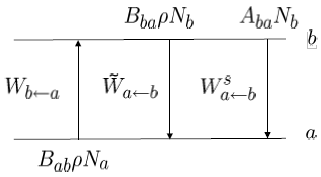
\includegraphics[scale=0.6]{ch2/image2}
	\captionof{figure}{ }
	\end{wrapfigure}
On peut (et en on parlera d'avantage dans la section suivante) faire le lien avec les coefficients
d'\textsc{Einstein}. Commentons les transitions ci-contre. Pour que la première flèche existe, il
faut que $N_a$ existe, mais également une densité de radiation $\rho$. Le coefficient $B_{ab}$ n'est
autre que le coefficient de proportionnalité donnant une probabilité. Il existe également le 
phénomène symétrique (seconde flèche) : il faut ici que $N_b$ soit peuplé et qu'il y ai une certaine
densité de radiations. La troisième flèche (émission spontanée) peut elle se produire sans radiation
à condition que le niveau $b$ soit peuplé.


\section{Lien avec les coefficients d'Einstein}
Écrivons l'équation cinétique du niveau $a$. La transition $a\to b$ dépeuple $a$ tandis que
la $b\to a$ le repeuple
\begin{equation}
\frac{dN_a}{dt} = - \frac{dN_b}{dt} =
- B_{ab} \rho(\omega_{ba}) N_a + B_{ba} \rho(\omega_{ba}) N_b
 + A_{ba} N_b
\end{equation}
A l'équilibre, $\frac{dN_a}{dt} = \frac{dN_b}{dt} = 0$. On peut en tirer un expression de $\rho$
\begin{equation}
\rho(\omega_{ba}) = 
\frac{A_{ba} }{B_{ab} (N_a/N_b) - B_{ba}}
\end{equation}
L'équation de \textsc{Boltzmann} (en oubliant les facteurs de dégénérescence) permet de déterminer
l'évolution du rapport $N_a/N_b$
\begin{equation}
\frac{N_a}{N_b} = e^{-(E_a - E_b)/kT} = e^{\hbar \omega_{ba} /kT}
\end{equation}
De son côté, \textsc{Planck} a proposé un expression pour la densité d'un corps noir
\begin{equation}
\rho(\omega_{ba})
= \frac{\hbar \omega_{ba}^3}{\pi^2 c^3}
\frac{1}{e^{\hbar \omega_{ba} /kT} -1  }
\end{equation}
\textsc{Einstein} avait les précédentes équations sous la main.  Il a remarqué - avec en plus 
l'équation de \textsc{Boltzmann} à disposition - que l'égalité entre son $\rho$ et celui trouvé par
\textsc{Planck} est vérifiée si les conditions si les conditions suivantes sont respectées
\begin{equation}
\left\{
\begin{array}{l}
B_{ab} = B_{ba} \\
A_{ba} = \frac{\hbar \omega_{ba}^3}{\pi^2 c^3} \; B_{ba}
\end{array} \right. \quad\Leftrightarrow\quad
 \left\{ \begin{array}{l}
B_{ab} = \frac{W_{b \leftarrow a}}{\rho} \\
A_{ba} = W^s_{a \leftarrow b}
\end{array} \right.
\end{equation}
\textsc{Interprétation manquante} (au pire, cf. \textit{Physique des lasers}).

\section{Spectre des atomes hydrogénoïdes}
Maintenant que nous avons établi la forme de l'élément matriciel, il serait intéressant de comprendre
comment celui-ci couple les états $n=2$ et $n=3$ par exemple. Pour se faire, reprenons la probabilité
de transition d'émission stimulée et spontanée($s$)
\begin{equation}
\begin{array}{ll}
W^{E1}_{b \leftarrow a} &\DS= \frac{4 \pi^2}{c \hbar^2} \left( \frac{e^2}{4 \pi \epsilon_0 } \right)
 I(w_{ba}) \vert  \hat{  \mbox{\boldmath $ \epsilon $}} \cdot 
{\bf  r}_{ba} \vert ^2\vspace{2mm}\\
W_{a \leftarrow b}^{E1,s}(\theta, \phi) \; d \Omega &\DS= 
\frac{1}{2 \pi \hbar c^3} \left( \frac{e^2}{4 \pi \epsilon_0} \right)
  \omega_{b a}^3
\vert  \hat{  \mbox{\boldmath $ \epsilon $}} \cdot 
{\bf  r}_{ba} \vert ^2 d \Omega
\end{array}
\end{equation}
Exprimons le vecteur polarisation $\hat{\vec{\epsilon}}$ en composantes sphériques
\begin{equation}
\left\{
\begin{array}{ll }
\epsilon^{(1)}_{+1}  & = - \frac{1}{\sqrt{2}} 
 \left( \hat{\epsilon}_x + i  \hat{\epsilon}_y \right) \\
\epsilon^{(1)}_{0}  & =  \hat{\epsilon}_z \\
\epsilon^{(1)}_{-1}  & = + \frac{1}{\sqrt{2}}
 \left(  \hat{\epsilon}_x - i  \hat{\epsilon}_y \right)
\end{array} \right.
\end{equation}
En faisant de même pour le vecteur $\vec{r}$
\begin{equation}
\left\{
\begin{array}{ll }
r^{(1)}_{+1}  & = - \frac{1}{\sqrt{2}} \left( x + i y \right) \\
r^{(1)}_{0}  & = z \\
r^{(1)}_{-1}  & = + \frac{1}{\sqrt{2}} \left( x - i y \right)
\end{array} \right.
\end{equation}
Ceci forme un tenseur sphérique irréductible d'ordre 1 (se transforme comme un vecteur par
rotation). A partir de deux tenseur, il est possible d'en tirer un tenseur scalaire. Il faut
pour cela faire un produit tensoriel des deux OTI
\begin{equation}
\left[ {\bf T}^{(k_1)} \times {\bf W}^{(k_2)} \right]^{(K)}_Q \equiv
\sum_{q_1,q_2} C(k_1k_2q_1q_2;KQ) \; T^{(k_1)}_{q_1} W^{(k_2)}_{q_2}
\end{equation}
En couplant des tenseurs sphériques irréductibles, il est possible de créer un tenseur irréductible
scalaire.

\subsubsection*{Parenthèse : symboles $3-j$}
Pour se faciliter la vie, on introduit les symboles $3-j$. Pour comprendre leur utilité, repartons
des coefficients de Clebsch-Gordon
\begin{equation}
C(j_1 j_2 m_1 m_2; J M) 
= ( j_1 j_2 m_1 m_2 \vert j_1 j_2 J M)= ( j_1 j_2 m_1 m_2 \vert  J M) 
= ( j_1 m_1 j_2 m_2 \vert  J M)
\end{equation}
Par \textbf{définition} des \textit{symboles $3-j$}
\begin{equation}
( j_1 j_2 m_1 m_2 \vert j_1 j_2 J M)
\equiv
(-1)^{j_1 - j_2 + M} [ J ]^{1/2} 
\left( \begin{array}{ccc} j_1 & j_2 & J \\ m_1 & m_2 & -M \end{array} 
\right) 
\end{equation}
L'utilité de ces symboles se trouve dans les propriétés de ceux-ci
\begin{equation}
\left( 
\begin{array}{ccc} j_1 & j_2 & j_3 \\ m_1 & m_2 & m_3 \end{array} 
\right) 
= 
\left( 
\begin{array}{ccc} j_2 & j_3 & j_1 \\ m_2 & m_3 & m_1 \end{array} 
\right)= (-1)^{j_1 + j_2 + j_3}
\left( 
\begin{array}{ccc} j_2 & j_1 & j_3 \\ m_2 & m_1 & m_3 \end{array} 
\right)
\end{equation}
Ceux-ci sont non nuls si
\begin{equation}
 \neq 0 \Rightarrow \left\{
\begin{array}{l}
\delta(j_1,j_2,j_3) \\
m_1 + m_2 + m_3 = 0
\end{array}  \right.
\end{equation}
Ce qui constitue une puissante règle de sélection.

\subsection{Produit scalaire de 2 OTI}
Construisons le produit scalaire entre deux OTI. Pour se faire, évaluons le produit entre deux
tenseurs suivant\footnote{Je n'ai pas de notes sur ce slide (20), si quelqu'un peut compléter}
\begin{equation}
\left[ T^{(k)} \times W^{(k)} \right]^{(0)}_0 \equiv
\sum_{q} 
\left( \begin{array}{ccc} k & k & 0 \\ -q & q & 0 \end{array} 
\right)  \; T^{(k)}_{-q} W^{(k)}_{q}
= (-1)^k [k]^{-1/2} \sum_q (-1)^q \; T^{(k)}_{-q} W^{(k)}_{q}
\end{equation}
On en tire l'expression du produit scalaire tensoriel\\

\cadre{
\begin{equation}
Q \equiv T^{(k)} \cdot W^{(k)} \equiv
\sum_q (-1)^q \; T^{(k)}_{-q} W^{(k)}_{q}
\end{equation}}\ \\

Nous avons comme probabilité de transition
\begin{equation}
W^{E1}_{b \leftarrow a} = \frac{4 \pi^2}{c \hbar^2} \left( \frac{e^2}{4 \pi \epsilon_0 } \right)
 I(w_{ba}) \vert  \hat{  \mbox{\boldmath $ \epsilon $}} \cdot 
{\bf  r}_{ba} \vert ^2
\end{equation}
Développons le produit scalaire se trouvant dans le module carré
\begin{equation}
\begin{array}{ll}
  \hat{  \mbox{\boldmath $ \epsilon $}} \cdot 
{\bf  r}_{ba}
&\DS= - \epsilon^{(1)}_{-1} \left( r^{(1)}_{+1} \right)_{ba} 
+ \epsilon^{(1)}_{0} \left(  r^{(1)}_{0} \right)_{ba}
- \epsilon^{(1)}_{+1}\left(  r^{(1)}_{-1} \right)_{ba}\vspace{2mm}\\
&\DS= +  \epsilon^{(1)\ast}_{+1}  \left( r^{(1)}_{+1} \right)_{ba} 
+  \epsilon^{(1)\ast}_{0}  \left(  r^{(1)}_{0} \right)_{ba}
+  \epsilon^{(1)\ast }_{-1}  \left(  r^{(1)}_{-1} \right)_{ba}\vspace{2mm}\\
&\DS= \sum_q \; \epsilon^{(1)\ast}_q I^q_{n'l'm';nlm}
\end{array}
\end{equation}
Dans l'atome d'hydrogène, $a$ et $n$ ne sont finalement qu'un \textit{set} de nombres quantiques.
Continuons en explicitant $I^q_{n'l'm';nlm}$
\begin{equation}
\begin{array}{ll}
I^q_{n'l'm';nlm} &\DS=  \sqrt{\frac{4 \pi}{3}} \int_0 ^\infty
\; dr \; r^3 R_{n'l'}(r)^\ast  R_{nl}(r)\times \int_0^{2 \pi} \int_0^{\pi}
Y^\ast_{l'm'} Y_{1q} Y_{lm} \sin \theta d\theta d\phi\vspace{2mm}\\
&\DS= \langle l' m' \vert C^{(1)}_q \vert l m  \rangle \int_0 ^\infty
\; dr \; r^3 R_{n'l'}(r)  R_{nl}(r)
\end{array}
\end{equation}
où l'on voit apparaître les harmoniques sphériques de l'opérateur. Explicitons cette fois 
$\langle l' m' \vert C^{(1)}_q \vert l m \rangle$
\begin{equation}
\langle l' m' \vert C^{(1)}_q \vert l m \rangle
= \sqrt{\frac{4 \pi}{3}} \int_0^{2 \pi} \int_0^{\pi}
Y^\ast_{l'm'} Y_{1q} Y_{lm} \sin \theta d\theta d\phi
= (-1)^{-m'} [l',l]^{1/2}
\left( \begin{array}{ccc} l' & 1 & l \\ 0 & 0 & 0 \end{array} \right)
\left( \begin{array}{ccc} l' & 1 & l \\ -m' & q & m \end{array} \right)
\end{equation}
Grâce à la propriété des coefficients $3-j$ énoncée ci-dessus, on en tire la \textbf{forte} 
règle de sélection suivante :\\

\cadre{\begin{equation}
 \neq 0 \Rightarrow \left\{
\begin{array}{l}
\delta(l',1,l) \\
(l' +1 + l)~\mbox{pair} \end{array} \right\} 
\Rightarrow \Delta l = l' - l = \pm 1
\end{equation}}\ \\

Le nombre quantique $l$ ne peut varier que d'au maximum \textbf{une} unité lors d'une transition.
On obtient finalement quelque chose de simple, à géométrie sphérique
\begin{equation}
-m' + q + m = 0 \Rightarrow
\left\{ \begin{array}{ll}
m' = m \; \; (\Delta m = 0) & \mbox{si}~q = 0 \\
m' = m \pm 1 \; \; (\Delta m = \pm 1) &\mbox{si}~q = \pm 1
\end{array} \right.
\end{equation}\ \\

A l'aide de l'explicitation de $\langle l' m' \vert C^{(1)}_q \vert l m \rangle$, on peut 
ré-écrire $I^q_{n'l'm';nlm}$
\begin{equation}
I^q_{n'l'm';nlm} =  \sqrt{\frac{4 \pi}{3}} \int_0 ^\infty
\; dr \; r^3 R_{n'l'}(r)^\ast  R_{nl}(r)\times \int_0^{2 \pi} \int_0^{\pi}
Y^\ast_{l'm'} Y_{1q} Y_{lm} \sin \theta d\theta d\phi
\end{equation}


\subsection{Lien de la règle de sélection $\Delta l = \pm 1$ avec la parité}
Nous avons
\begin{equation}
\phi_{ n l m }(r, \theta, \phi) = R_{nl} (r) Y_{lm} (\theta, \phi)
\end{equation}
A l'aide de l'opérateur parité
\begin{equation}
\hat{I} \phi_{ n l m }({\bf r}) = 
\hat{I} R_{nl} (r) Y_{lm} (\theta, \phi)
\equiv 
\phi_{ n l m }( - {\bf r})=
R_{nl} (r) Y_{lm} (\pi - \theta, \phi + \pi)
=  (-1)^l R_{nl} (r) Y_{lm} (\theta, \phi)
\end{equation}
En en tire que
\begin{equation}
\begin{array}{ll}
I^q_{n'l'm';nlm} &\DS=  (-1)^{l' + 1 + l}  I^q_{n'l'm';nlm}\\
&\DS \neq 0 ~\mbox{si}~(l' +1 + l)~\mbox{pair} 
\end{array}
\end{equation}
En résumé, l'inversion ne touche que la partie sphérique. Si $l$ est pair la parité sera impaire
et paire inversement. On en déduit qu'une\textbf{transition E1 ne peut relier que des états de
parité différentes}. La règle $\Delta l=\pm1$ est la \textit{règle de }\textsc{Laporte}. Le
\textit{slide 23} représente les transitions à l'aide de cette règle de sélection tandis que 
le \textit{slide 24} les classe par parité.


\section{Force de raie, force d'oscillateur et temps de vie}
Le théorème de \textsc{Wigner-Eckart} est apprécié pour les règles de sommes extraordinaires
des $3-j$ mais aussi pour ses règles de sélection.\\

\theor{\textsc{Wigner-Eckart}\ 
\begin{equation}
\langle \alpha j m \vert T^{(k)}_q \vert \alpha' j' m' \rangle
= (-1)^{j-m} \left( \begin{array}{ccc}
j  &  k  &  j'  \\ -m  &  q  &  m' \end{array} \right) 
\langle \alpha j \Vert {\bf T}^{(k)} \Vert \alpha' j' \rangle
\end{equation}}\ \\

Chaque élément de matrice peut s'écrire comme un élément de matrice réduit multiplié par un
$3-j$. Ré-écrivons alors l'élément de matrice qui nous intéresse sous cette forme
\begin{equation}
 \langle l m_l \vert C^{(1)}_q \vert l'm_l' \rangle =
(-1)^{l-m_l} \left( \begin{array}{ccc}
l  &  1  &  l'  \\ -m_l  &  q  &  m_l' \end{array} \right) 
\langle  l \Vert {\bf C}^{(1)} \Vert l' \rangle
\end{equation}
L'élément de matrice réduit s'écrit
\begin{equation}
\langle  l \Vert {\bf C}^{(1)} \Vert l' \rangle
= (-1)^l [l,l']^{1/2} \left( \begin{array}{ccc}
l  &  1  &  l'  \\ 0  &  0 &  0 \end{array} \right)
\end{equation}
Énonçons la fabuleuse \textbf{règle de somme}
\begin{equation}
\sum_{mm'}  \vert
\langle \alpha j m \vert T^{(k)}_q \vert \alpha' j' m' \rangle \vert ^2
= \vert \langle \alpha j \Vert {\bf T}^{(k)} \Vert \alpha' j' \rangle \vert ^2 
\sum_{mm'} \left( \begin{array}{ccc}
j  &  k  &  j'  \\ -m  &  q  &  m' \end{array} \right) ^2 
=  \frac{1}{2k+1} \vert \langle \alpha j \Vert {\bf T}^{(k)} \Vert \alpha' j' \rangle \vert ^2
\end{equation}


\subsection{Force de raie et force d'oscillateur}
Appliquons la règle de somme et utilisons une notation plus efficace
\begin{equation}
S(\alpha J, \alpha' J' ) = \sum_{MM'q} \vert \langle \alpha JM \vert \mu^{(1)}_q  \vert \alpha J' M' \rangle \vert^2= 
\vert \langle \alpha J \Vert 
\mbox{\boldmath $ \mu $}^{(1)} \Vert \alpha J' \rangle \vert^2
\end{equation}
Suite au cours de demain!

\iffalse
unité atomique de moment dipolaire au carré. C'est (e*a0)^2 l'unité de ça

303.7 : nombre quand S exprime en u.a., quand lamda est en 1. il faut... pour calculer un nombre sans dimension

nombre sans dim qui va introduire la force d'oscillateur. EN injectant çala dedans on trouve 1. g_k c'est facteur de dégen
\fi
























%%%%%%%%%%%%%%%%%
% Bibliographie %
%%%%%%%%%%%%%%%%%
%\newpage
%\chapter{Bibliographie}
%\nocite{*}
%\printbibliography[heading=none]

%%%%%%%%%%%
% Annexes %
%%%%%%%%%%%
\appendix
%\input{annexes/annexe1.tex}


\end{document}
